\documentclass[11pt,letterpaper]{article}
\usepackage{templates/emnlp2016/emnlp2016}
\usepackage{times}
\usepackage{latexsym}

% Uncomment this line for the final submission:
\emnlpfinalcopy

%  Enter the EMNLP Paper ID here:
\def\emnlppaperid{***}

% To expand the titlebox for more authors, uncomment
% below and set accordingly.
% \addtolength\titlebox{.5in}

\newcommand\BibTeX{B{\sc ib}\TeX}

%%%%%% MY Addition %%%%
\usepackage{booktabs}
\usepackage{soul, color}
\usepackage[unicode=true]{hyperref}
\usepackage{graphicx}
%%%%%%%%%%%%%%%%%


% % \usepackage{lmodern}
% % % \usepackage{amssymb,amsmath}
% \usepackage{ifxetex,ifluatex}
% \usepackage{fixltx2e} % provides \textsubscript
% \ifnum 0\ifxetex 1\fi\ifluatex 1\fi=0 % if pdftex
%   \usepackage[T1]{fontenc}
%   \usepackage[utf8]{inputenc}
% % \else % if luatex or xelatex
%   \ifxetex
%     \usepackage{mathspec}
%     \usepackage{xltxtra,xunicode}
%   \else
%     \usepackage{fontspec}
%   \fi
%   \defaultfontfeatures{Mapping=tex-text,Scale=MatchLowercase}
%   \newcommand{\euro}{€}
% % % % % % \fi
% % use upquote if available, for straight quotes in verbatim environments
% \IfFileExists{upquote.sty}{\usepackage{upquote}}{}
% % use microtype if available
% \IfFileExists{microtype.sty}{%
% \usepackage{microtype}
% \UseMicrotypeSet[protrusion]{basicmath} % disable protrusion for tt fonts
% }{}
% % \ifxetex
%   \usepackage[setpagesize=false, % page size defined by xetex
%               unicode=false, % unicode breaks when used with xetex
%               xetex]{hyperref}
% \else
%   \usepackage[unicode=true]{hyperref}
% \fi
% \usepackage[usenames,dvipsnames]{color}
% \hypersetup{breaklinks=true,
%             bookmarks=true,
%             pdfauthor={A. Aziz Altowayan and Lixin Tao Pace University Computer Science Department New York, USA \{aa10212w, ltao\}@pace.edu},
%             pdftitle={Evaluating Word Similarity Measure of Embeddings Through Binary Classification},
%             colorlinks=true,
%             citecolor=blue,
%             urlcolor=blue,
%             linkcolor=magenta,
%             pdfborder={0 0 0}}
% \urlstyle{same}  % don't use monospace font for urls
% %  \usepackage{natbib}
%  \usepackage[authoryear,round,longnamesfirst]{natbib}
   \usepackage[square, numbers]{natbib} % use square brackets 
%  \bibliographystyle{plainnat}
  \bibliographystyle{unsrtnat} % maintain order of appeareance https://tex.stackexchange.com/a/213577/81376
% % % \usepackage{graphicx,grffile}
\makeatletter
\def\maxwidth{\ifdim\Gin@nat@width>\linewidth\linewidth\else\Gin@nat@width\fi}
\def\maxheight{\ifdim\Gin@nat@height>\textheight\textheight\else\Gin@nat@height\fi}
\makeatother
% % Scale images if necessary, so that they will not overflow the page
% % margins by default, and it is still possible to overwrite the defaults
% % using explicit options in \includegraphics[width, height, ...]{}
% \setkeys{Gin}{width=\maxwidth,height=\maxheight,keepaspectratio}
\setkeys{Gin}{width=80mm,height=\maxheight,keepaspectratio}
% % % \setlength{\parindent}{0pt}
% \setlength{\parskip}{6pt plus 2pt minus 1pt}
% \setlength{\emergencystretch}{3em}  % prevent overfull lines
\providecommand{\tightlist}{%
  \setlength{\itemsep}{0pt}\setlength{\parskip}{0pt}}
% % \setcounter{secnumdepth}{0}
% 


\title{Evaluating Word Similarity Measure of Embeddings Through Binary
Classification}
\author{A. Aziz Altowayan and Lixin Tao\\
Pace University\\
Computer Science Department\\
New York, USA\\
{\{aa10212w, ltao\}@pace.edu}\\}
\date{}
%
% % Redefines (sub)paragraphs to behave more like sections
% \ifx\paragraph\undefined\else
% \let\oldparagraph\paragraph
% \renewcommand{\paragraph}[1]{\oldparagraph{#1}\mbox{}}
% \fi
% \ifx\subparagraph\undefined\else
% \let\oldsubparagraph\subparagraph
% \renewcommand{\subparagraph}[1]{\oldsubparagraph{#1}\mbox{}}
% \fi

\begin{document}
\maketitle
\begin{abstract}
We consider the following problem: given neural language models
(embeddings) each of which is trained on an unknown data set, how can we
determine which model would provide a better result when used for
feature representation in a downstream task such as text classification
or entity recognition? In this paper, we assess the word similarity
measure through analyzing its impact on word embeddings learned from
various datasets and how they perform in a simple classification task.
Word representations were learned and assessed under the same
conditions. For training word vectors, we used the implementation of
Continuous Bag of Words described in {[}1{]}. To assess the quality of
the vectors, we applied the analogy questions test for word similarity
described in the same paper. Further, to measure the retrieval rate of
an embedding model, we introduced a new metric (Average Retrieval Error)
which measures the percentage of missing words in the model. We observe
that scoring a high accuracy of syntactic and semantic similarities
between word pairs is not an indicator of better classification results.
This observation can be justified by the fact that a domain-specific
corpus contributes to the performance better than a general-purpose
corpus. For reproducibility, we release our experiments scripts and
results.\footnote{https://github.com/iamaziz/w2v-eval}
\end{abstract}

% pandoc-xnos: macro to create a caption without a prefix
\makeatletter
\long\def\@makenoprefixcaption#1#2{
  \vskip\abovecaptionskip
  \sbox\@tempboxa{#2}
  \ifdim \wd\@tempboxa >\hsize
    #2\par
  \else
    \global \@minipagefalse
    \hb@xt@\hsize{\hfil\box\@tempboxa\hfil}
  \fi
  \vskip\belowcaptionskip}
\makeatother

% pandoc-fignos: save original macros
\makeatletter
\let\@oldmakecaption=\@makecaption
\let\oldthefigure=\thefigure
\let\oldtheHfigure=\theHfigure
\makeatother

% pandoc-fignos: environment disables figure caption prefixes
\makeatletter
\newcounter{figno}
\newenvironment{no-prefix-figure-caption}{
  \let\@makecaption=\@makenoprefixcaption
  \renewcommand\thefigure{x.\thefigno}
  \renewcommand\theHfigure{x.\thefigno}
  \stepcounter{figno}
}{
  \let\thefigure=\oldthefigure
  \let\theHfigure=\oldtheHfigure
  \let\@makecaption=\@oldmakecaption
  \addtocounter{figure}{-1}
}
\makeatother

\section{Introduction}\label{introduction}

Language modeling is the crux of the problem in Natural Language
Processing (NLP. Recently, neural language models have outperformed the
traditional language model approaches such as \emph{n}-gram. The
superiority of the neural methods lies in their capability to overcome
the curse of the dimensionality problem while, simultaneously, capturing
different similarities between words \citep{Goodfellow-et-al-2016}.

Neural language models learn distributed representations for each word
in the form of real-numbers-value vectors, which allows similar words to
have similar vectors. Such sharing is an important characteristic that
enables the learning model to treat related words similarly and, hence,
gives the model the ability to generalize. These word representations
are usually known simply as \emph{Word Embeddings}.

Nowadays, word embedding is the standard approach for feature
representation in many NLP tasks. Traditional feature representation
methods, such as bag-of-words and term frequency--inverse document
frequency (TFIDF), rely on hand-crafted feature extractor, and are
time-consuming and domain-specific. Hence, embedding based techniques
provide a better alternative for automating many tasks in language
modeling and NLP.

Among these techniques context-predicting semantic vectors have
distinctly proven their superiority to the count-based ones
\citep{baroni2014don}. While count-based vectors are more about the
frequency of the word, context-based vectors make more emphasis on the
word and its context.

Popular word vector learning methods are introduced in
{[}\citep{Mikolov:2013wc}, \citep{Pennington:2014uw},
\citep{Manning:2015kh}{]} and have gained great attention since then.
From these methods, learning continuous word embeddings using skip-gram
and negative sampling is the most common approach for building word
vectors \citep{ling2015two}. This method was introduced and described in
\citep{Mikolov:2013wc}.

However, since vectors training occurs in an unsupervised fashion, there
is no accurate way to estimate the quality of the vector representations
objectively. Several extrinsic and intrinsic evaluation methods have
been discussed in \citep{bakarov2018survey}. Nonetheless, at the time of
this writing, there is still no reliable method for comparing the
quality of different embedding models. So, this is still an open
question. Commonly, the quality can be assessed using the word
similarity task, which is a test with a set of similarity analogy
questions \citep{Mikolov:2013wc}.

Nevertheless, with the current word similarity evaluation method, word
similarity accuracy and having more vocabulary in the model do not
result in better performance in the downstream task.

From experiments, we show that scoring well on word similarity measure
questions does not imply better performance in the downstream task. Our
findings are in line with the observations of
\citep{faruqui2016problems}. Therefore, we observe that the accuracy of
word similarity measure is not, necessarily, an indicator for the
usefulness of the word embedding model. In this paper, we explain and
justify this claim based on the observation of our experimentation
results.

For instance, we show that the GoogleNews embedding model has the
following two advantages over IMDB model. First, it scores better
results in word similarity accuracy (74.26\%) in comparison to IMDB's
(23.71\%); second, GoogleNews contains 3 million vocabulary words while
IMDB contains around 19,000. Despite these advantages of GoogleNews, the
classifiers' performance was worse with GoogleNews than with IMDB.

The rest of the paper is structured into the following parts: related
work, our experiments, discussion, future work, and finally, the
conclusion.

\section{Related Work}\label{related-work}

We approached related work in the following manner: first, we
investigated what it takes to build quality embedding models and which
components to consider. We then analyzed similar work for evaluating
word embeddings using extrinsic and intrinsic methods. We also reviewed
the available current work on building domain-specific embeddings. And
finally, we look into work that focuses on the syntactic and semantic
similarities between words.

Training elements such as the model, the corpus, and the parameters have
been analyzed in detail in \citep{lai2016generate}. They observed that
the corpus domain is more important than its size. This explains our
results where the smaller domain-specific corpus (IMDB) achieved better
results than the much larger general-purpose corpus (GoogleNews).

We reviewed papers on evaluating word vectors' quality and model
accuracies. Existing evaluation methods fall into two types: intrinsic
and extrinsic evaluation. In the intrinsic evaluation, the goal is to
directly assess the quality of word vectors in hopes that it will
reflect on the performance of the downstream tasks. So, synthetic
metrics are proposed to test the semantic and syntactic similarities
between words.

For example, a pre-selected set of query terms is used to estimate
words' relationships. Each query denotes two pairs of ``analogically''
similar words. For example, relation \emph{big} to \emph{bigger} in the
same way as as \emph{small} to \emph{smaller} is called ``syntactic
similarity'', while relating \emph{Tokyo} to \emph{Japan} in the same
way as \emph{London} to \emph{England} is called ``semantic
similarity''). Then, such queries can take the form of questions, for
instance, ``What is the word similar to \emph{small} in the same sense
as \emph{bigger} is similar to \emph{big}?''. To query the model, a
question is formulated in an algebraic expression as follows:
\emph{answer = vector(`bigger') - vector(`big') + vector(`small')}. This
method was first proposed in \citep{Mikolov:2013wc}; and published with
a set of around 20 thousand syntactic/semantic questions. It is fast and
computationally inexpensive, however, there are problems associated with
this technique \citep{faruqui2016problems}. Further, other evaluation
techniques have been proposed to reduce bias
\citep{schnabel2015evaluation}. In such methods, they directly compare
embeddings with respect to specific queries.

While in the extrinsic evaluation, we indirectly evaluate word
embeddings. In other words, we use the embeddings as input features to a
downstream task and measure the performance metrics specified to that
task \citep{schnabel2015evaluation}. For instance, when the task is text
classification, we would use the embeddings to represent words in the
text. In some approaches, they applied extrinsic evaluations to learn
task-specific embeddings \citep{tang2014learning}.

Finally, a thorough investigation and survey covering the current
evaluation methods have been discussed in \citep{bakarov2018survey}.

\section{Building Word Embeddings}\label{building-word-embeddings}

\subsection{Data Collection and
Exploration}\label{data-collection-and-exploration}

The diagram in fig. \ref{fig:workflow} illustrates the overall workflow
of our experiment.



\begin{figure}
\centering
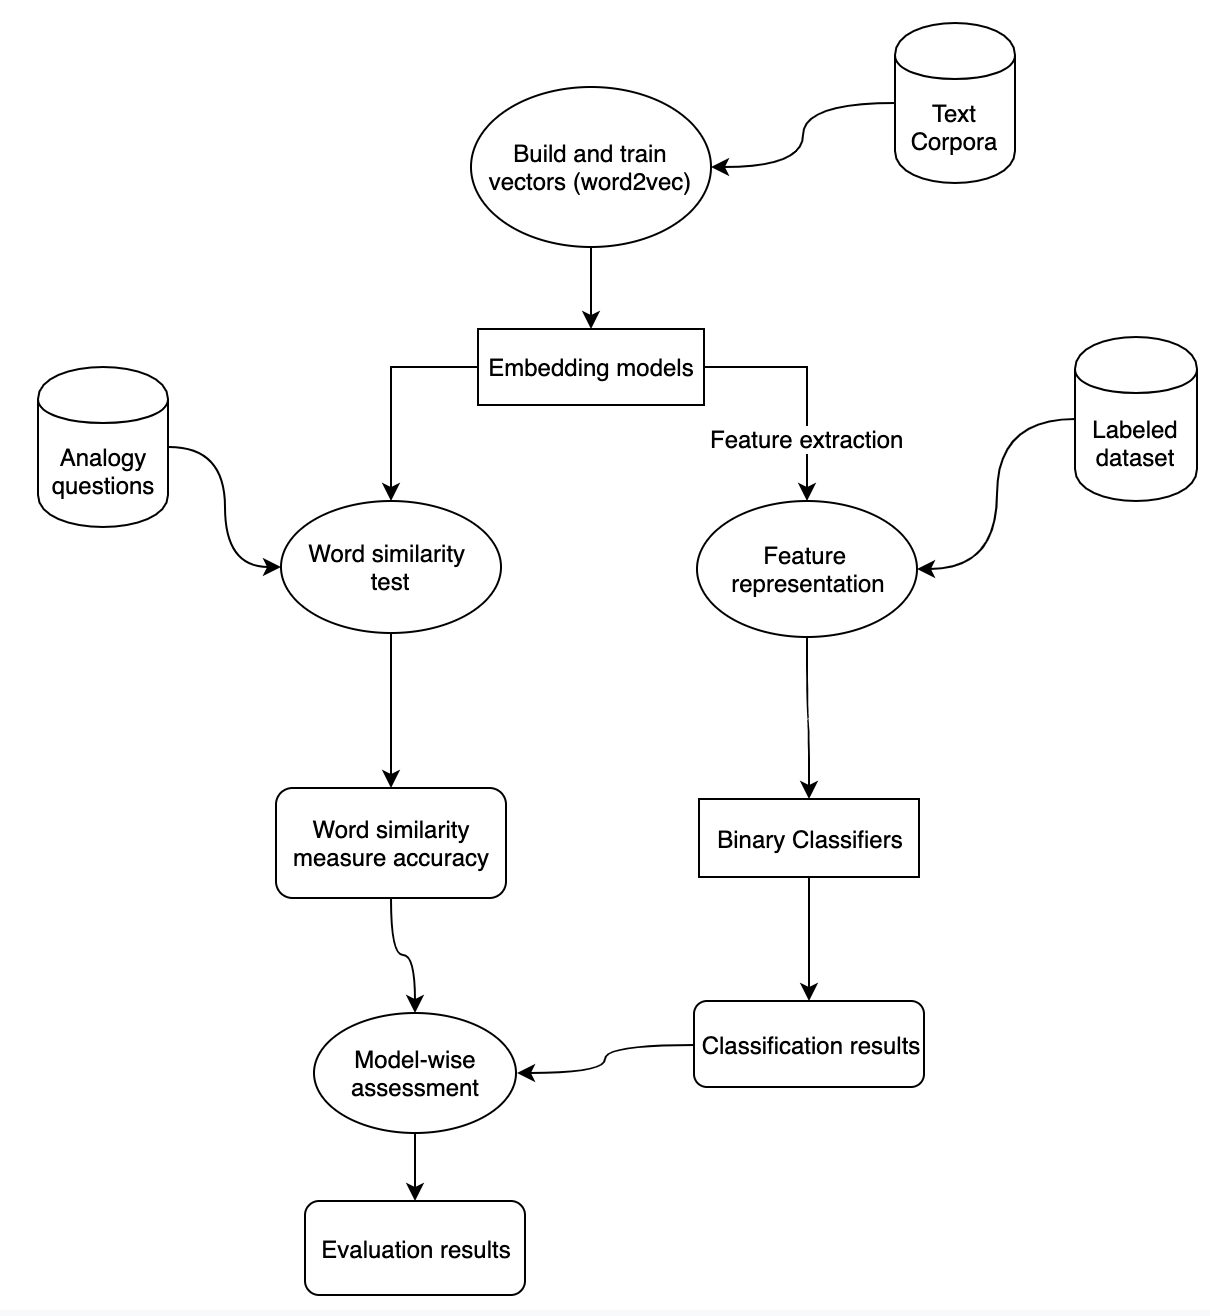
\includegraphics{img/w2v_eval_workflow.png}
\caption{The approach design and workflow\label{fig:workflow}}
\end{figure}



In this section, we describe the data sources and texts we used for
training the embedding models. We started with two well-known corpora.
The first one is text8, a standard
corpus\footnote{http://mattmahoney.net/dc/textdata} used in NLP
community which has around 100MB of cleaned English text of a Wikipedia
dump from 2006, and the second one is the Large Movie Review Dataset (or
IMDB\footnote{http://ai.stanford.edu/~amaas/data/sentiment/}). IMDB
contains 100 thousand movie reviews prepared for sentiment
classification problems. Later on, we will use this same dataset in our
classification experiment; we are aware this may cause bias in the
datasets, further discussion to follow later.

As a way to augment our data, we created a new hybrid corpus by
concatenating the above two corpora; we call it \emph{text8-imdb}. This
allows us to compare the results of two models and their hybrid to see
how they may affect one another. Later on, in the classification
section, we will see that \emph{imdb} achieved the best among the three.
This is a bit surprising, because its \emph{average retrieval error}
(1.46) was higher than that of \emph{text8-imdb} (0.99); though it still
achieved better results.

For additional insights about the data, we explored each corpus for
statistical information ``meta-data'' such as number of the unique
words, the total count of characters, and the total count of words. See
table \ref{tbl:corpora_stats} for more details on these metrics.

\begin{table*}[ht]
\centering
\footnotesize

\begin{tabular}{@{}l||ccc@{}}
\toprule

Corpus & char count & word count & unique words \\\midrule

imdb & 125,882,839 & 23,573,192 & 144,841 \\
text8 & 100,000,000 & 17,005,207 & 253,854 \\

\bottomrule
\end{tabular}

\caption{Statistics of the training text (corpus).
\label{tbl:corpora_stats}}

\end{table*}

We also wanted to get a better sense of the characters' usage and their
frequency in each corpus. Figure \ref{fig:cp-letter-freq} illustrates
some visualization of the usages. It shows the frequency of the 26
English letters usage in each of the three corpora.



\begin{figure}
\centering
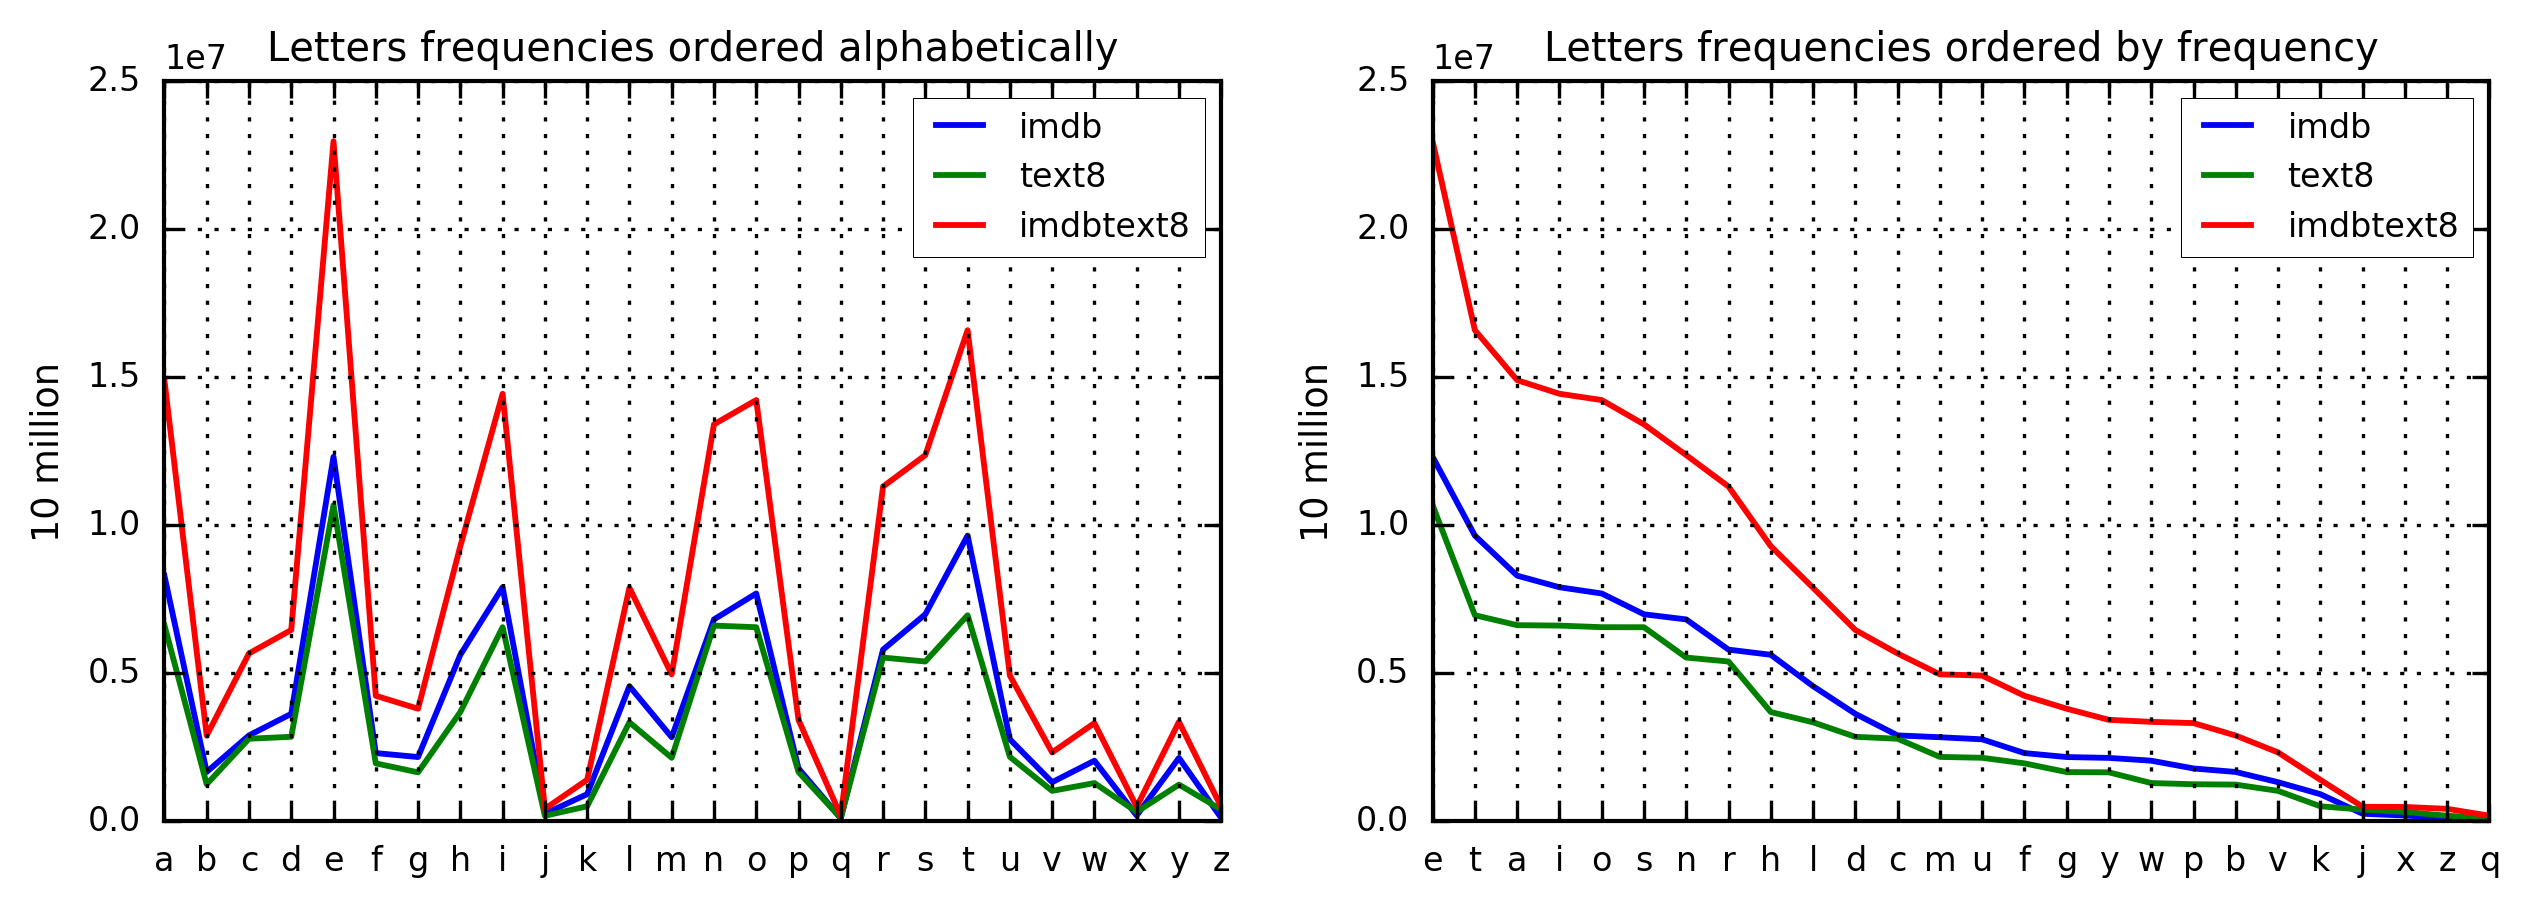
\includegraphics{img/cp-letter-freq.png}
\caption{Letters frequencies as they appear in text8 and
IMDB\label{fig:cp-letter-freq}}
\end{figure}



\subsection{Model Training and
Parameters}\label{model-training-and-parameters}

Following \citep{Mikolov:2013wc} approach for learning vector
representations of words, we trained three models using three various
corpora. In the first one, we merged the entire set of 100,000 movie
reviews \citep{maas2011learning} into one big text file, we will refer
to the vectors ``model'' generated from this text as \textbf{imdb}. And
for the second model, as mentioned in the previous section, we used a
100 MB of cleaned Wikipedia English text known as \emph{text8}, we will
call the model from this corpus: \textbf{text8}. The third ``hybrid''
model is the combination of the two above files (as one big text file).
We refer to this model as \textbf{imdb-text8}. The fourth model, in our
experiment, is \textbf{GoogleNews}. A pre-trained model published in
\citep{Mikolov:2013wc}.

With the exception of
GoogleNews\footnote{It was not clear to us which exact parameters were used. See: Mikolov's response in word2vec-gmail-group},
all the models were trained using CBOW architecture with the same
hyper-parameters. We used the original (C language) implementation of
word2vec toolkit\footnote{https://github.com/tmikolov/word2vec}. After
compiling and building the software locally, we use the following
command to train the models:

\begin{verbatim}
$ ./word2vec -train $CORPUS \
             -output $OUT \
             -cbow 1 \
             -size 300 \
             -window 10 \
             -negative 25 \
             -hs 0 \
             -sample 1e-4 \
             -threads 20 \
             -binary 1 \
             -iter 15
\end{verbatim}

\subsection{Exploring Models}\label{exploring-models}

After we built the models, we decided to evaluate their response to the
analogy question test sets. 
Table \ref{tbl:embed_stats} displays the number of the learned ``vectorized'' vocabulary in each model. 
The table also shows the number of questions seen in the model,
along with their average similarity accuracy. These results were
obtained based on \texttt{\$\ ./word2vec/compute-accuracy} script in the
same toolkit. For faster approximate evaluation, we used the recommended
threshold of 30,000 to reduce vocabulary.

\begin{table*}[ht]
\centering
\footnotesize

\begin{tabular}{@{}ccccc@{}}
\toprule

Embeddings & \# vocab. & dim. & \# quest. seen & avg. sim.
acc. \\\midrule

imdb & 53,195 & 300 & 10,505 & 33.41\% \\
text8 & 71,291 & 300 & 12,268 & 53.60\% \\
imdb-text8 & 94,158 & 300 & 12,448 & 59.89\% \\
GoogleNews & \textbf{3M} & 300 & \textbf{13,190} & \textbf{76.85\%} \\

\bottomrule
\end{tabular}

\caption{Statistics of the models' and their results on the analogy
questions test. \label{tbl:embed_stats}}

\end{table*}

\subsection{Determining Models
Accuracy}\label{determining-models-accuracy}

To conduct a fair comparison between models, we introduce the
\emph{Average Retrieval Error} ``AVG\_ERR'' as a way to estimate the
vectors' availability in the given model. It is the total number of
\emph{missed words} (i.e.~words that queried but not available in the
embedding model) over the \emph{total words} queried. See formula
\ref{eq:error} below:

\begin{equation}\frac{ \sum_{i=1}^{n}Q({t_i - r_i})}{ n }\label{eq:error}\end{equation}

Where, \(Q\) is a query to the model which returns the vectors for a set
of given tokens (words), \(n\) is the total number of the queries made,
\(t\) is the number of tokens in query \(i\), and \(r\) is the number of
retrieved (found) vectors for query \(i\).

For simplicity, we can rewrite \ref{eq:error} as:

\begin{equation}Avg.\;Retrieval\;Error = \frac{ \sum_{i=1}^n{m_i} } { n }\label{eq:avg_error}\end{equation}

And \(m\) is the number of missed (not found) vectors for query \(i\).

In figure \ref{fig:question_seen}, we show the number and percentage of
analogy questions seen in the model (with a threshold of 30K) for word
similarity task.



\begin{figure}
\centering
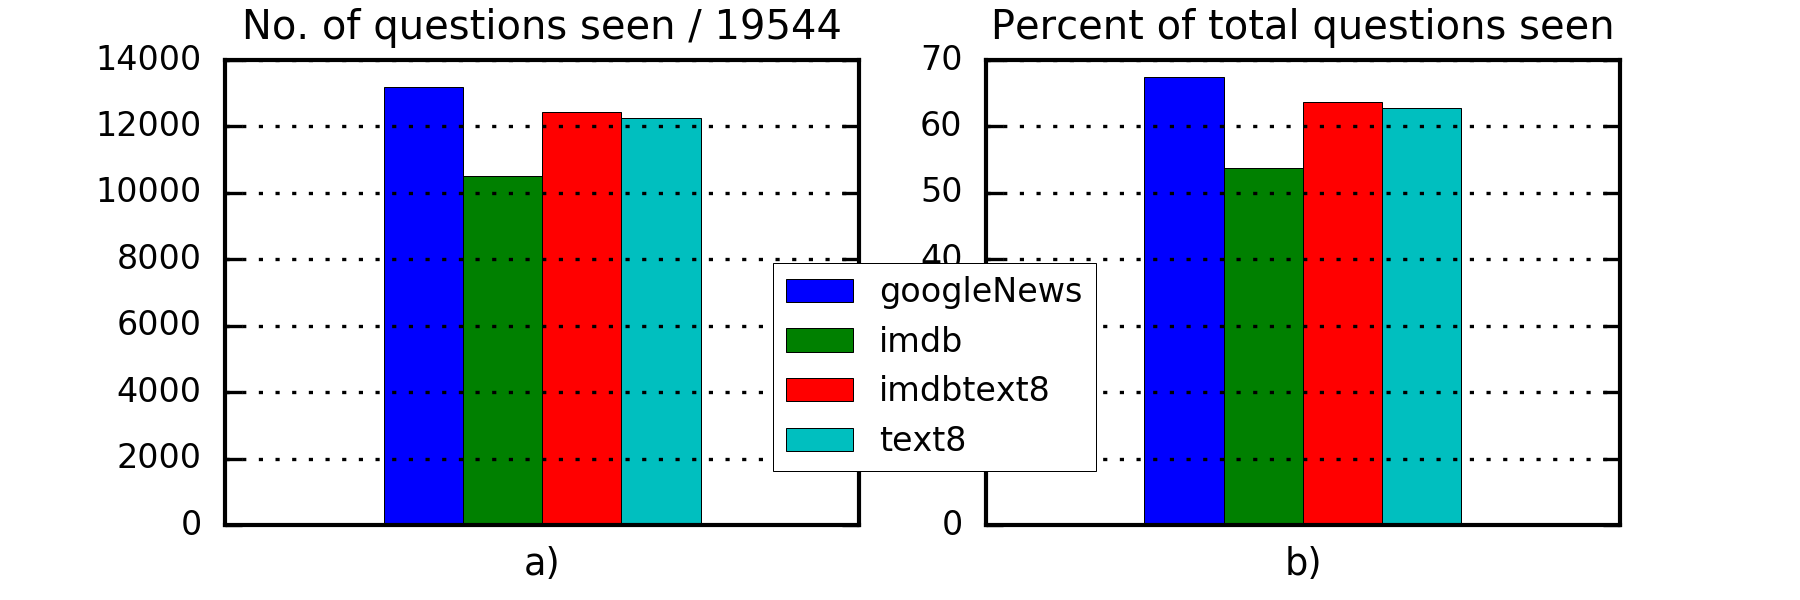
\includegraphics{img/em-questions.png}
\caption{Embeddings results on the word analogy task (out of the total
19544 questions), fig. a. is the number of questions seen and fig. b. is
the percentage of the questions seen.\label{fig:question_seen}}
\end{figure}



We also recorded the accuracy for each topic of the 14 question type
categories. Instead of using a huge table with many numbers, we decided
to illustrate the result in figure \ref{fig:topics_acc} to quickly grasp
the topics' results.

\begin{figure}
\centering
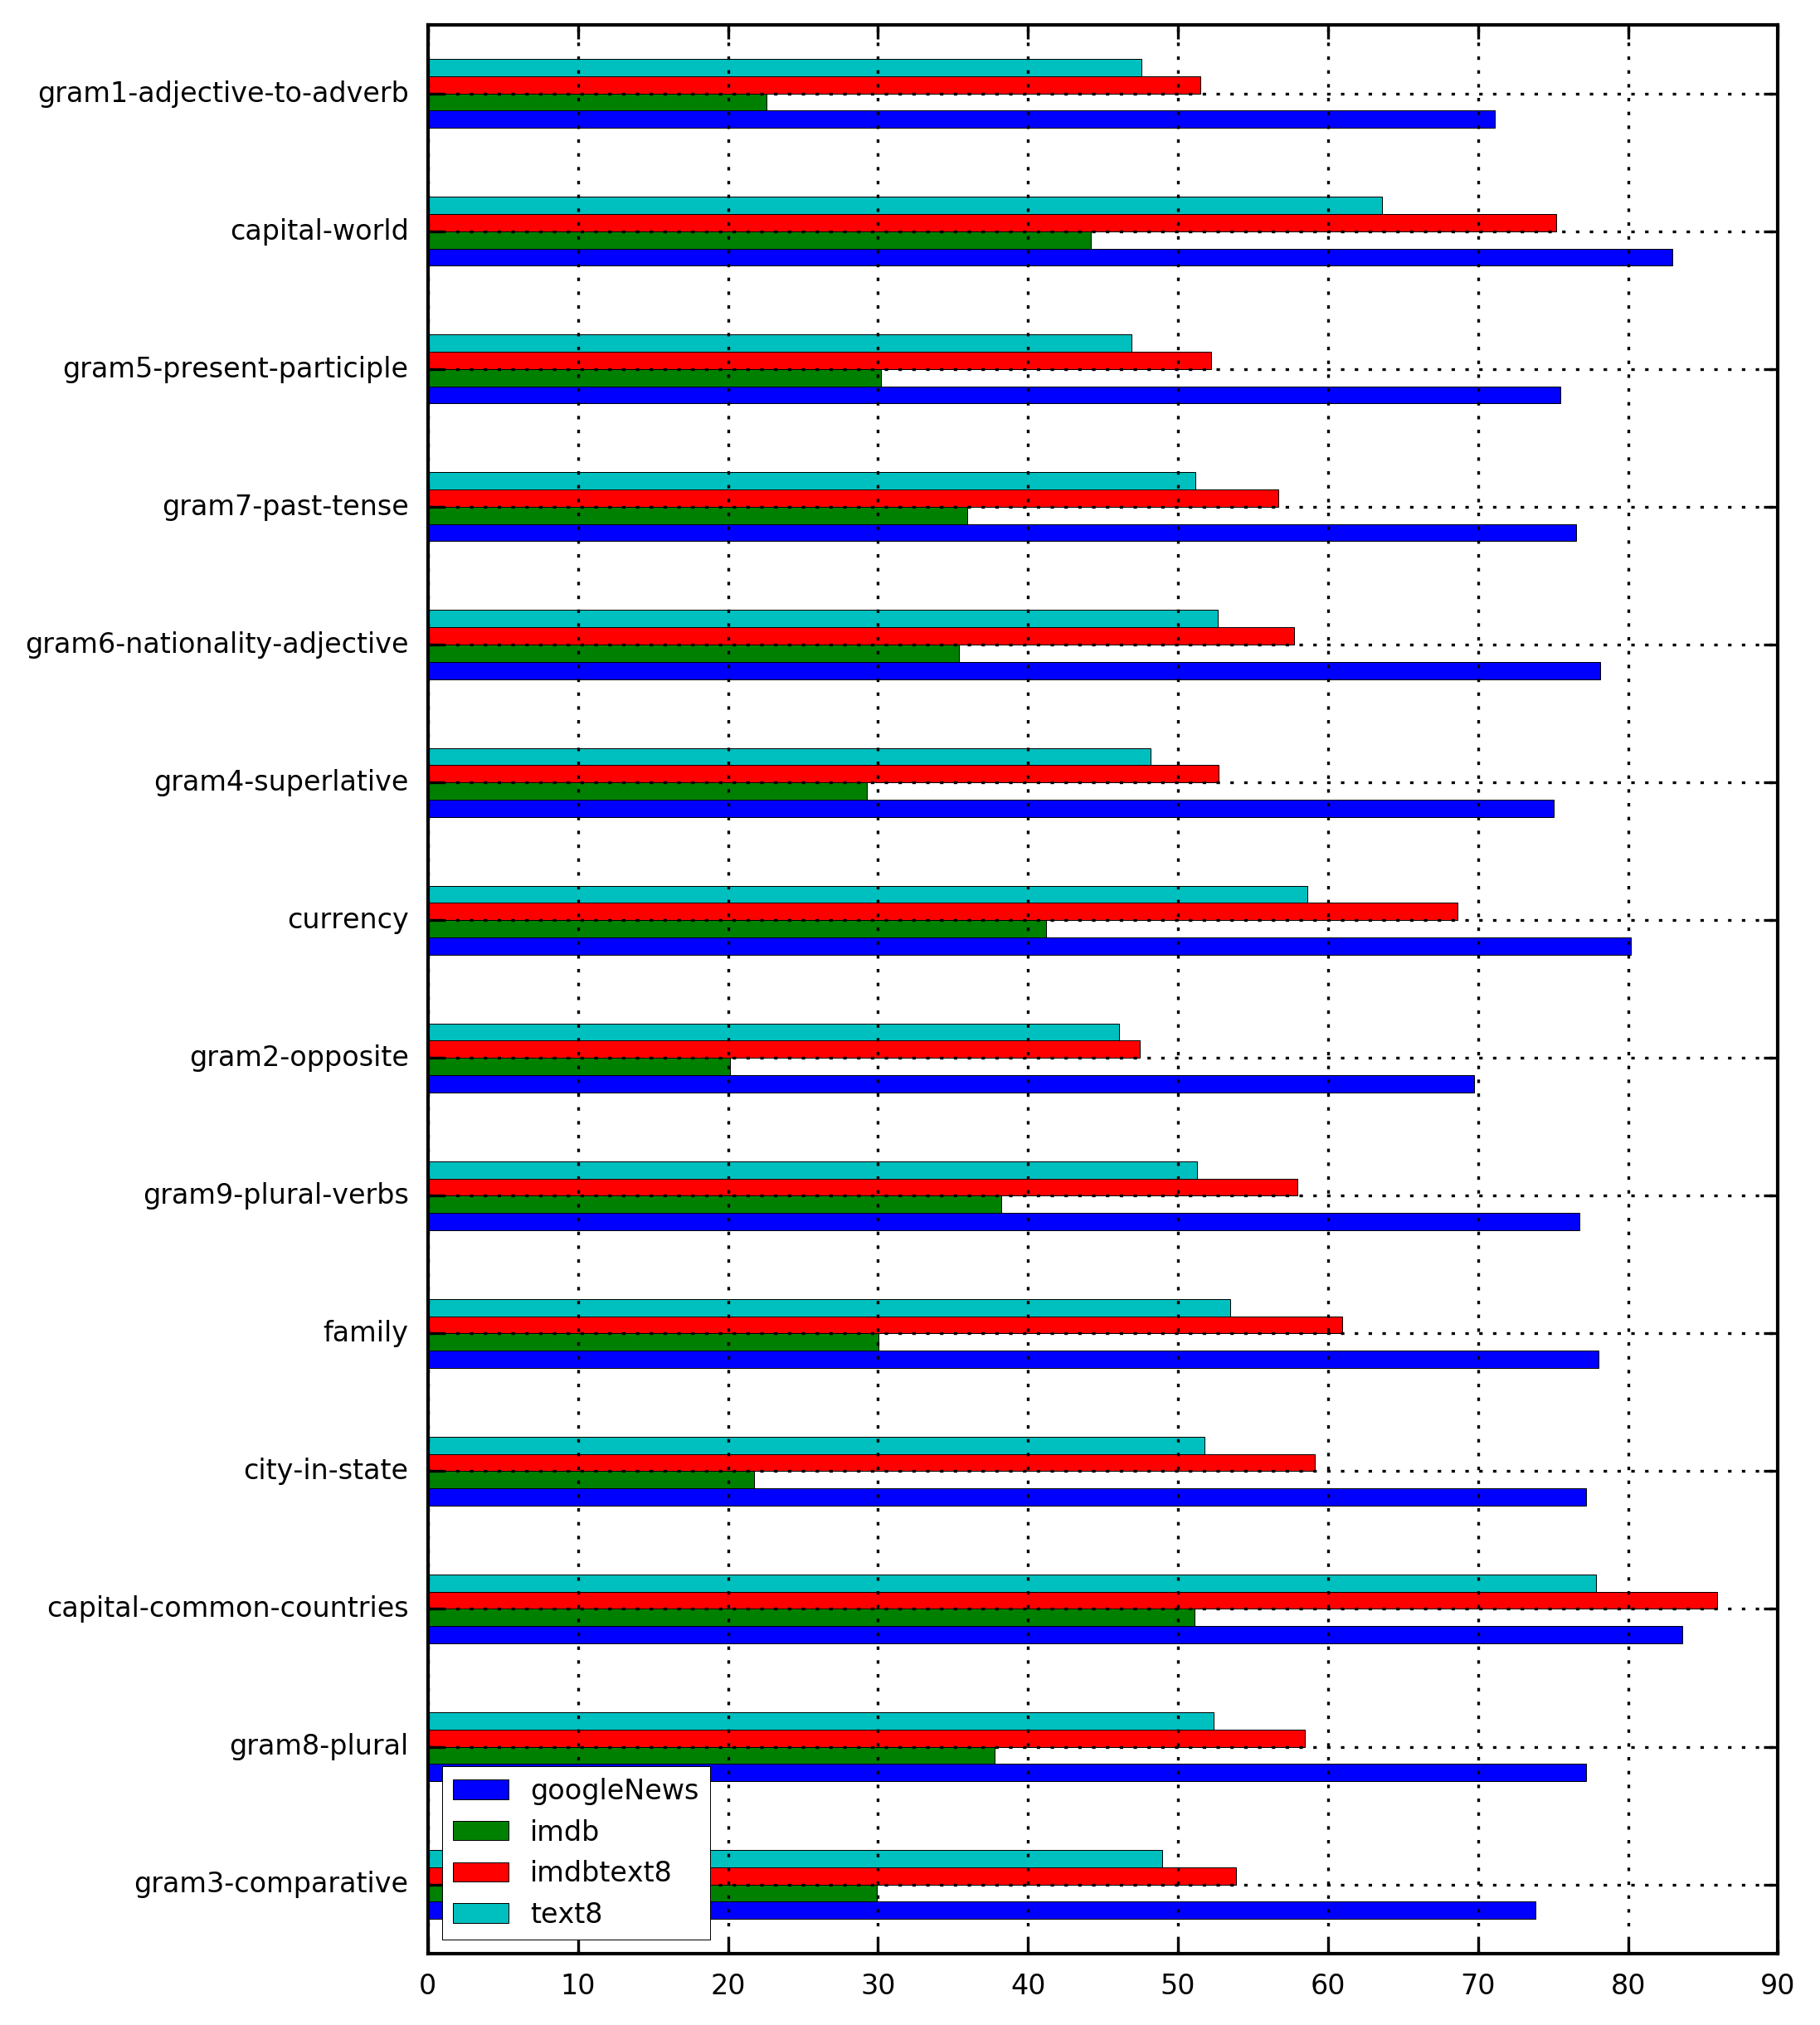
\includegraphics[width=65mm]{img/em-topics-acc.png}
\caption{Topic-wise results of the models' accuracy on word analogy
task}
\label{fig:topics_acc}
\end{figure}

Finally, in figure \ref{overall_analogy}, we show the overall accuracy
results for every model; such as the average score for all topics and
density of topics' results.

\begin{figure*}[htbp]
\centering
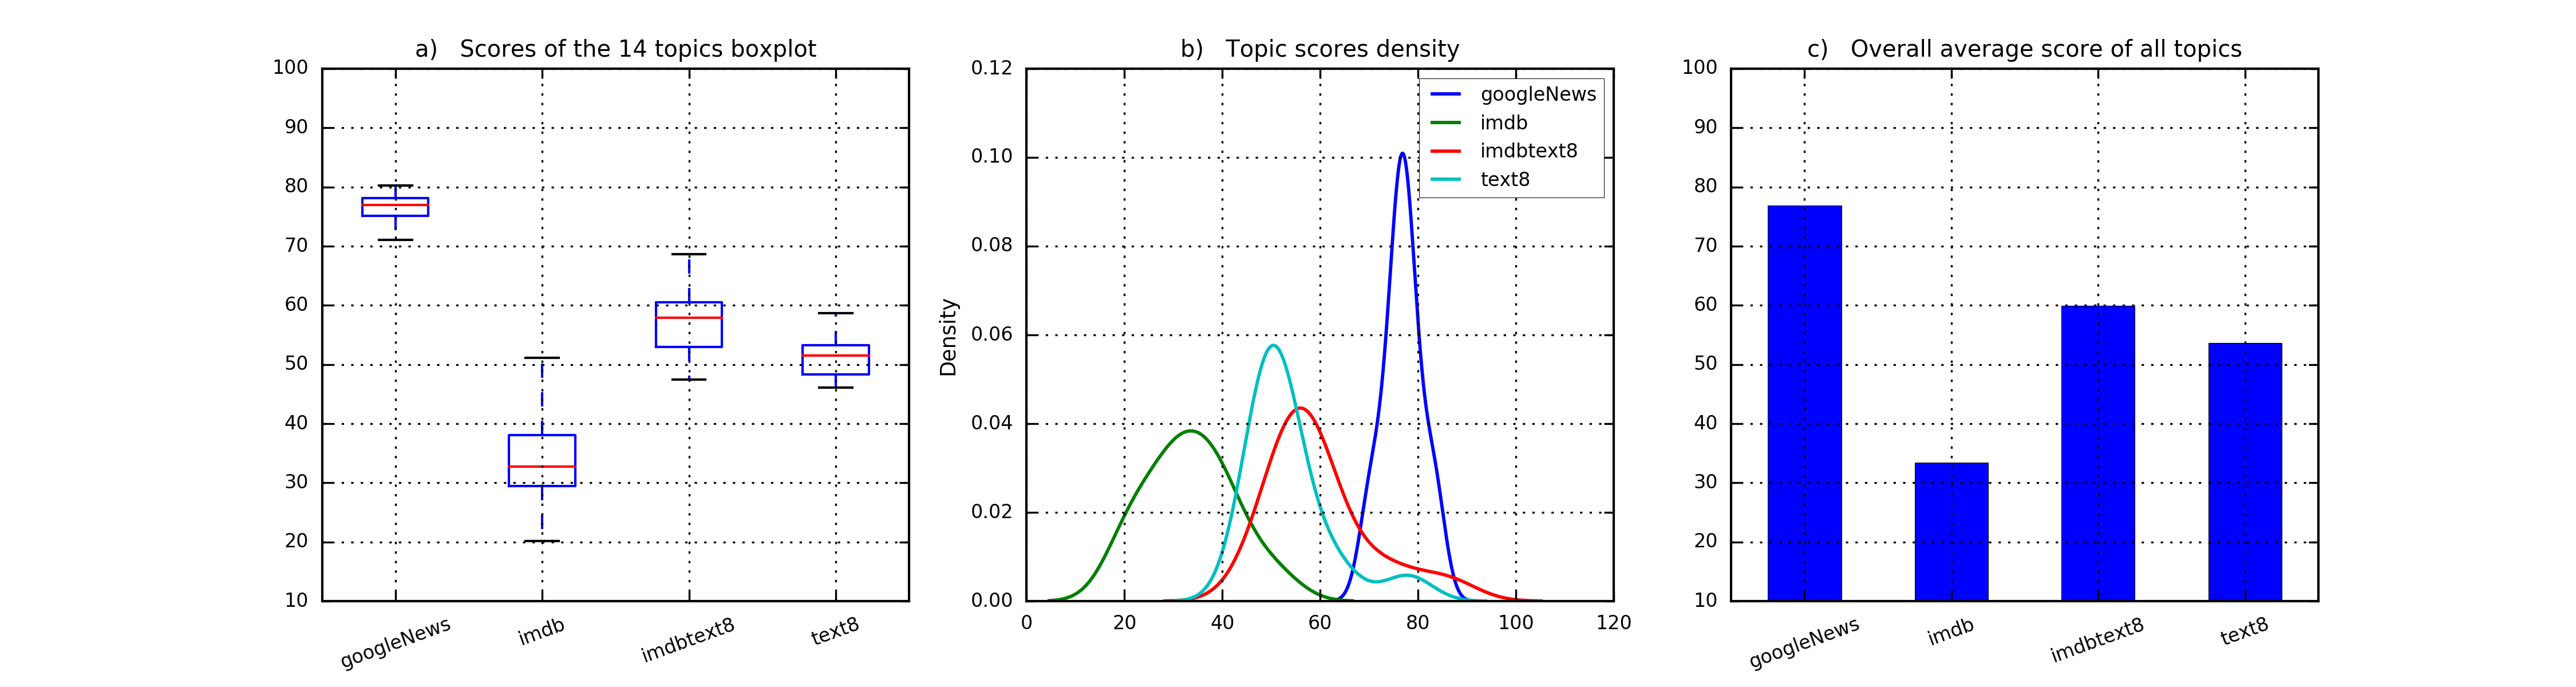
\includegraphics[width=160mm]{img/em-overall.png}
\caption{Visualizations of the overall models' performance in the analogy questions test}
\label{overall_analogy}
\end{figure*}

Despite the scored word similarity accuracy of the IMDB model, its
classification result is quite impressive. We will see that in the next
section; where the learned word representations reflect a great deal of
the actual semantics.

\section{Applying Embedding Models for Binary
Classification}\label{applying-embedding-models-for-binary-classification}

In this section we evaluate the performance of each embedding model in a
downstream task. Our task is a simple binary classification for
sentiment analysis problem.

\subsection{Supervised Training
Dataset}\label{supervised-training-dataset}

To train the sentiment classifiers, we used the popular benchmark
IMDB-50K movie reviews dataset. It was introduced by
\citep{maas2011learning}, and available to download.\footnote{\url{http://ai.stanford.edu/~amaas/data/sentiment/}}
The dataset, which was prepared specially for binary sentiment
classification, contains 25K highly polar movie reviews for training and
25K for testing. The sentiment of reviews is balanced in both data sets,
i.e.~one half is positive, and the other half is negative.

Additionally, IMDB has another unlabeled dataset contains 50K reviews
which we used in training our word2vec models. This dataset, however,
was not used for training the binary classifiers.

\subsection{Representing Reviews}\label{representing-reviews}

After preprocessing the review text, the vector representation of each
token ``word'' is then retrieved by querying the embedding model. If a
token is not found in the embeddings' vocabulary, its representation
will be ignored. That's where the concept of \emph{Average Retrieval
Error} comes from. The more tokens missed, the higher the average error
will be. When all the review's tokens are processed, the review then
will be represented as a fixed size feature vector by averaging the
representations of all tokens.

\subsection{Training Classifiers
Results}\label{training-classifiers-results}

We trained five simple binary classification algorithms Perceptron,
Support Vector Machines, Stochastic Gradient Descent, Logistic
Regression, and Random Forest. We used the built-in implementations of
these algorithms provided by the scientific toolkit library
``scikit-learn''\footnote{https://scikit-learn.org}. As for parameters
tuning, we applied the default parameters in scikit-learn.

To know the complete set of parameters for each classifier, one can
refer to the log file we included with our project code.

\begin{table*}[ht]
\centering
\footnotesize

\begin{tabular}{@{}l||l||l||ccccc@{}}
\toprule

Model & Vocab. & AVG\_ERR & Percept. & SVM & SGD & LogReg & RForest \\\midrule

imdb & 53,195 & 1.46 & \textbf{84.29\%} & \textbf{89.20\%} & \textbf{86.49\%} & \textbf{89.19\%} & \textbf{84.39\%} \\
text8 & 71,291 & 4.62 & 76.62\% & 81.17\% & 75.44\% & 81.22\% & 73.88\% \\
imdb-text8 & 94,158 & \textbf{0.99} & 80.11\% & 89.12\% & 85.50\% & 89.08\% & 83.96\% \\
GoogleNews & \textbf{3,000,000} & 28.04 & 78.94\% & 86.14\% & 82.89\% & 86.08\% & 80.16\% \\

\bottomrule
\end{tabular}

\caption{Vocabulary Size, Average Retrieval Errors, and Classifiers
Performance with each model. \label{tbl:classifiers_acc}}

\end{table*}

In table \ref{tbl:classifiers_acc}, we show the performance of each
classifier with each of the respective four embedding models.
For a better visual comparison of the same scores, see fig. \ref{fig:sentiment_score}. We can see that the classifiers scored better with IMDB embedding model, despite that GoogleNews model has better accuracy in
term of analogy query test. We can also notice that IMDB is still better
than its hybrid model text8-imdb which intuitively should enrich the
model's representation capacity by adding more vocabulary (which can be
verified by inspected the average retrieval error decrease from imdb to
text8-imdb). Reducing AVG\_ERR did not improve the classifiers; but on
the contrary, combining text8 degrades imdb's performance.

\begin{figure}
\centering
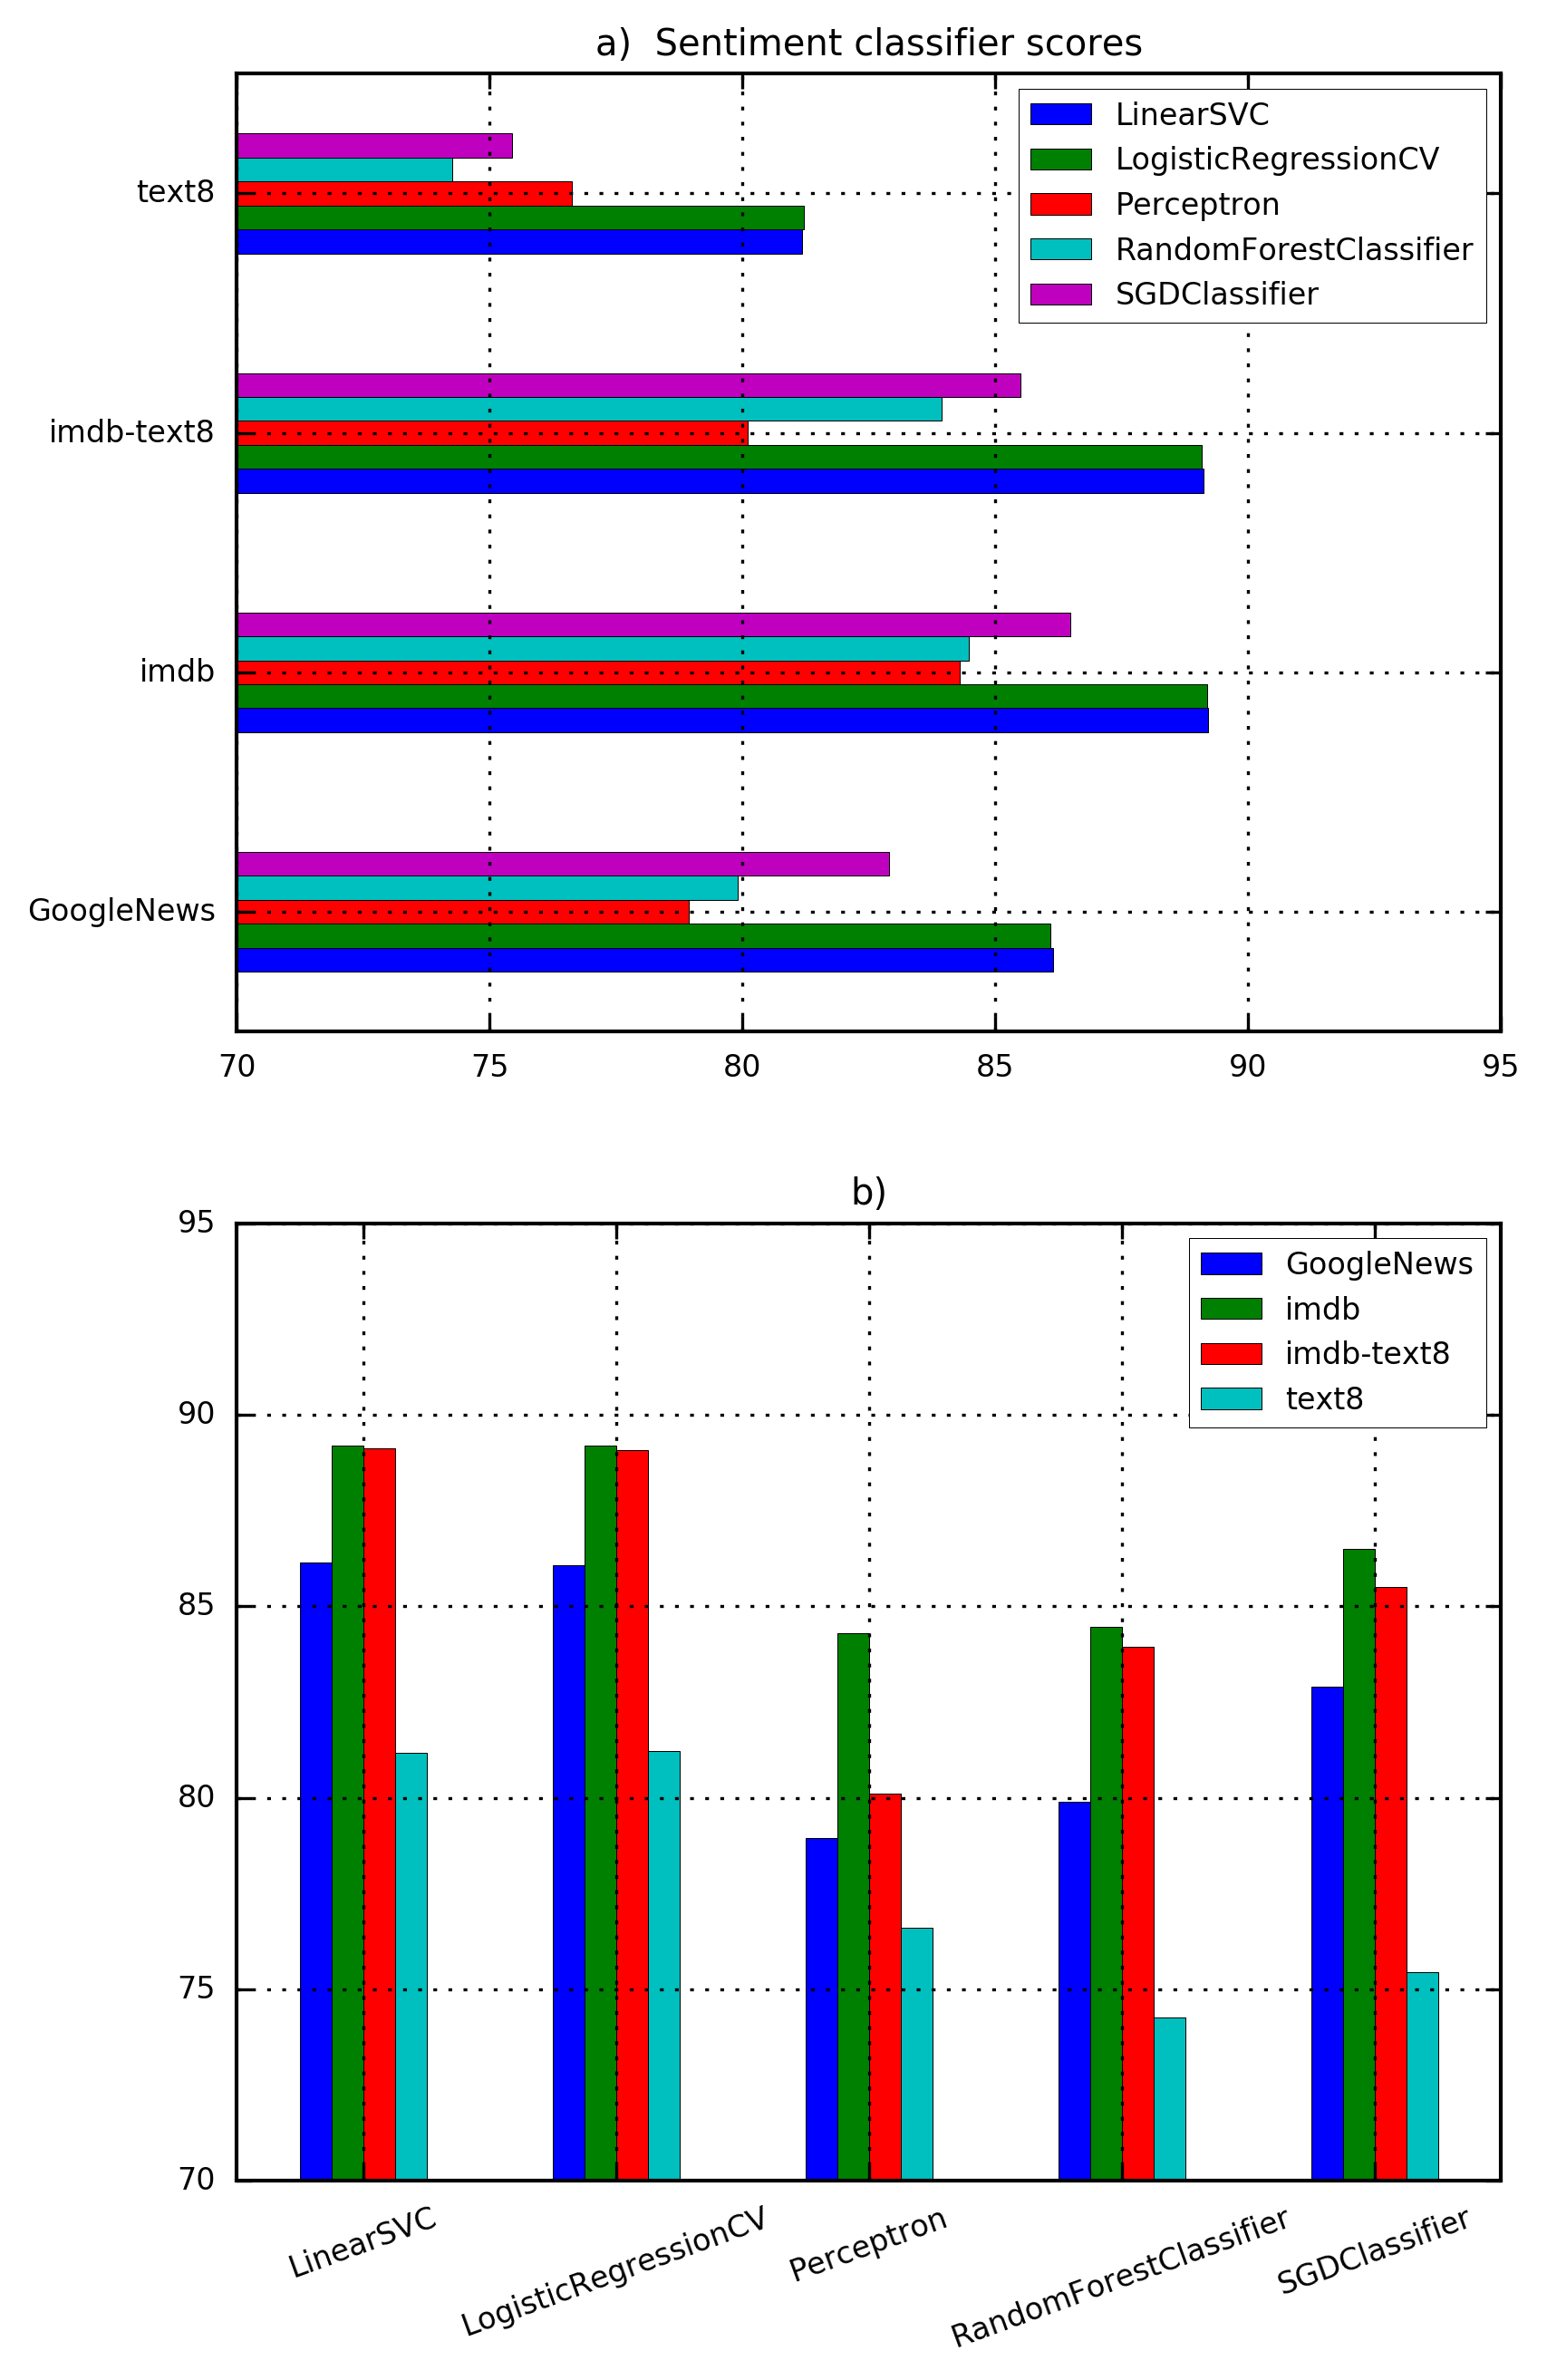
\includegraphics[width=65mm]{img/sent-clfs-score3.png}
\caption{Sentiment classifiers score with each embeddings. a) embedding models wise results, and b) classifiers wise results.}
\label{fig:sentiment_score}
\end{figure}

\textbf{Avoiding bias in IMDB}.  The training and testing datasets are initially the same corpus that we
use to generate imdb embeddings. Thus, and to make sure that our testing
is not biased, we used another sentiment dataset (i.e.~other than IMDB
reviews) to test the performance of the classifier. The dataset contains
7086 labeled (positive/negative) training sentences and 33052 unlabeled
sentences provided for prediction problems. We used the training data
for testing our classifiers, as we were not able to acquire the actual
labels of prediction set. As expected, the highest scores of the
classifiers still achieved with imdb embeddings.

\section{Results and Discussion}\label{results-and-discussion}

\textbf{Results summary}. To summarize and aggregate all the results and scores for both the intrinsic and extrinsic evaluations together in one place,
we took the average score of all classifiers achieved with each
embedding model. These aggregates are displayed in table \ref{tbl:summary}.

\begin{table*}[ht]
\centering
\footnotesize

\begin{tabular}{@{}l||l||ccc@{}}
\toprule

Embeddings & vocab. size & AVG. retrieval err. & AVG. similarity
acc. & AVG. sentiment score \\\midrule

imdb & 53,195 & 1.46 & 33.41\% & \textbf{86.73\%} \\
text8 & 71,291 & 4.62 & 53.60\% & 77.74\% \\
imdb-text8 & 94,158 & \textbf{0.99} & 59.89\% & 85.55\% \\
GoogleNews & \textbf{3M} & 28.04 & \textbf{76.85\%} & 82.79\% \\

\bottomrule
\end{tabular}

\caption{Summary on the final results for embedding models' accuracy and
classification performance \label{tbl:summary}}

\end{table*}

\textbf{Model Accuracy and Classifiers Performance}. Why IMDB word
embedding model is better than GoogleNews embedding? Learning
task-specific vectors through fine-tuning offers further gain in
performance. See static vs.~non-static representation (section 4.2 of
CNN sentence classification \citep{kim2014convolutional}).

So, for example, you'd expect words like ``amazing'' and ``awful'' to be
very far apart whereas in word2vec they'd probably be closer because
they can appear in similar contexts
\footnote{see: cnn-text-classification-tf Denny Britz's blog}.

In the accuracy evaluation, IMDB model scored 22.94\% on the 8182 test
cases found (out of the 19544 test cases); while the GoogleNews model
scored 74.26\% on the 7614 test cases found. Although the IMDB model
scored less, the sentiment classifiers performed better with it in
comparison to the other model.

\textbf{Improving classifiers' performance}. Although we were not
concerned with improving the overall performance of the classifiers,
there are several things to consider that can improve the classifiers'
results.

For example, one can apply the ensemble approach, described in
\citep{Mesnil:2014ti}, that combine multiple baseline models rather than
relying on a single model. Further improvement might be introduced by
describing the review feature differently, instead of averaging the
vectors \citep{lebret2015sum}.

Also, while training the vectors, careful choice and tuning of the
hyper-parameters could bring much gain to the model accuracy
\citep{Levy:2015us}. Finally, one may consider words dependency instead
of relying solely on linear contexts \citep{grefenstette2014deep}.

\textbf{Missing data}. When a given token (of a sentence) is not
available in the embedding model, its vector value is ignored. However,
it is counted toward the sentence length when we take the overall
average. Can we do something else about this? e.g.~1) substitute
(compute) its value as the average of other tokens in the same review,
or 2) do not count it in review length, or 3) apply other known
techniques for handling NaN values.

\textbf{Average retrieval error}. After comparing the models'
sensitivity to the average retrieval error, we noticed that word
retrieval in a model does not affect the overall performance. Possibly,
one way to enrich this metric is by introducing word-wise weights. For
example, common words can have low weight while the less common ones can
have higher weight.

\textbf{Extending this work}. We can think of three possible ways to
further extend this work. Firstly, expand the models range for broader
comparison. For instance, one can integrate more (other) pre-trained
models such as GloVe, ELMo, BERT to use in both experiments; embedding
quality assessment, and binary classifiers. Secondly, and to enrich the
procedure of classification comparison, one can try another approach to
aggregating the sentence features (other than averaging vectors for
sentence representations). Finally, in this work, we introduced the
\emph{Average Retrieval Error} ``AVG\_ERR''. We think this measure can
be further improved by adding weights to words in the sentences. For
example, stop words, and common vocabulary can have less weight than
those that are more specific.

\section{Conclusion}\label{conclusion}

We discussed the problem of choosing between multiple word embedding
models. To this end, we made the following contributions. We built and
trained three different embeddings models based on published data sets.
We, then, implemented two types of evaluation methods on the models. For
the intrinsic evaluation, we applied the word similarity measure method;
while we did the extrinsic evaluations through a binary classification
problem. We presented the results of performance comparisons over four
different embedding models. We also introduced a metric for measuring
the model's retrieval rate to the number of queries made. For
reproducibility, we released the models, data, and scripts used in our
experiments.

We have shown that scoring high accuracy in the Word Similarity Measure
test does not imply better performance in the downstream task. In other
words, if a model \emph{A} achieves a higher score than model \emph{B}
in the analogy question test, this does not mean \emph{A} will perform
better than \emph{B} in a downstream task. This finding is in line with
observations from related work. We also observed that the model's
coverage of vocabulary (i.e.~vocabulary size) is not as essential as
containing a domain-specific dictionary.

\bibliography{/Users/Aziz/Dropbox/thesis/myref.bib}

\end{document}
